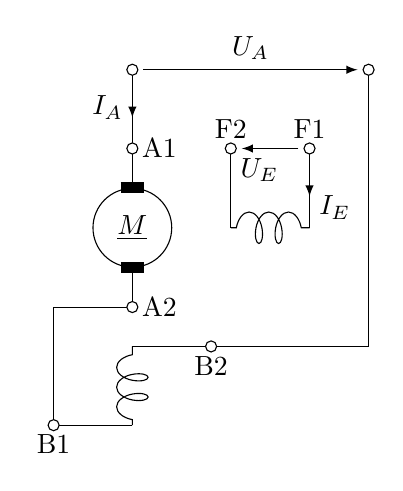
\begin{tikzpicture}
%
\node[circle,minimum width = 1cm,fill = white,draw](motor) at (0,0) {$\underline{M}$};
%
%Buersten
\draw [line width = 4pt] ([xshift = -0.15cm]motor.north) -- ([xshift = 0.15cm]motor.north);
\draw [line width = 4pt] ([xshift = -0.15cm]motor.south) -- ([xshift = 0.15cm]motor.south);
%
%Wicklungen: Wendepolwicklung und Reihenschlusserregerwicklung
\draw (motor.south) -- ([xshift=0cm,yshift = -0.5cm]motor.south) --
			([xshift=-1cm,yshift = -0.5cm]motor.south) -- ([xshift=-1cm,yshift = -2cm]motor.south) --
			([xshift= 0cm,yshift = -2cm]motor.south);
\draw decorate[decoration={name = coil,pre length = 2pt,post length = 2pt,segment length=2.5mm,amplitude=2mm}] 
			{([xshift= 0cm,yshift = -2cm]motor.south) --([xshift=0cm,yshift = -1cm]motor.south)};			
\draw	([xshift=0cm,yshift = -1cm]motor.south) -- ([xshift=1cm,yshift = -1cm]motor.south);
%
\draw ([xshift=1cm,yshift = -1cm]motor.south) -- ([xshift=3cm,yshift = -1cm]motor.south) -- ([xshift=3cm,yshift = 1.5cm]motor.north);
%
\draw ([xshift=0cm,yshift = 0cm]motor.north) -- ([xshift=0cm,yshift = 1.5cm]motor.north);		
%
%Erregerwicklung#
%
\draw ([xshift=1.25cm,yshift = 0.5cm]motor.north) --
			([xshift=1.25cm,yshift = 0cm]motor.center);
\draw decorate[decoration={name = coil,pre length = 2pt,post length = 2pt,segment length=2.5mm,amplitude=2mm}] 
			{([xshift= 1.25cm,yshift = 0cm]motor.center) --([xshift=2.25cm,yshift = 0cm]motor.center)};			
\draw	([xshift=2.25cm,yshift = 0cm]motor.center) -- ([xshift=2.25cm,yshift = 0.5cm]motor.north);		
%
%UA
\draw [-latex,shorten <= 4pt,shorten >=4pt] ([xshift = 0cm,yshift = 1.5cm]motor.north) -- 
([xshift = 1.5cm,yshift = 1.5cm]motor.north) node [above] {$U_{\text{A}}$} -- ([xshift = 3cm,yshift = 1.5cm]motor.north);
%
%IA
\draw [-latex,shorten <= 4pt,shorten >=4pt] ([xshift = 0cm,yshift = 1.5cm]motor.north) -- 
([xshift = 0cm,yshift = 0.75cm]motor.north) node [above left] {$I_{\text{A}}$};

%UE
\draw [-latex,shorten <= 4pt,shorten >=4pt] ([xshift = 2.25cm,yshift = 0.5cm]motor.north) -- 
([xshift = 1.25cm,yshift = 0.5cm]motor.north) node [below right] {$U_{\text{E}}$};
%
%IE
\draw [-latex,shorten <= 4pt,shorten >=4pt] ([xshift = 2.25cm,yshift = 0.5cm]motor.north) -- 
([xshift = 2.25cm,yshift = -0.25cm]motor.north) node [right] {$I_{\text{E}}$};


%
%Anschluesse
%
\filldraw[fill = white] ([yshift = 0.5cm]motor.north) circle (2pt) node[right] {A1};
\filldraw[fill = white] ([yshift = -0.5cm]motor.south) circle (2pt) node[right] {A2};

\filldraw[fill = white] ([xshift = -1cm,yshift = -2cm]motor.south) circle (2pt) node[below] {B1};
\filldraw[fill = white] ([xshift = 1cm,yshift = -1cm]motor.south) circle (2pt) node[below]{B2};
%
\filldraw[fill = white] ([xshift= 2.25cm,yshift = 0.5cm]motor.north) circle (2pt) node[above] {F1};
\filldraw[fill = white] ([xshift= 1.25cm,yshift = 0.5cm]motor.north) circle (2pt) node[above] {F2};
%
\filldraw[fill = white] ([yshift = 1.5cm]motor.north) circle (2pt);
\draw[fill = white] ([xshift = 3cm,yshift = 1.5cm]motor.north) circle (2pt);
%
\end{tikzpicture}